%
%  Proxies
%
%  Created by Tom Van Cutsem on 2010-01-18.
%  Copyright (c) 2010 Google. All rights reserved.
%
%\documentclass{acm_proc_article-sp}
\documentclass{sig-alternate}

% Use utf-8 encoding for foreign characters
%\usepackage[utf8]{inputenc}

% Setup for fullpage use
%\usepackage{fullpage}

% Multipart figures
%\usepackage{subfigure}

\usepackage{multirow}
% \usepackage{rotating} % for \begin{sidewaystable}
\usepackage{url}
\usepackage{mdwlist}

% Package for including code in the document
\usepackage{listings}
\lstdefinelanguage{javascript}{
   morekeywords={break,do,instanceof,typeof,case,else,new,var,catch,finally,return, void, continue, for, switch, while, debugger, function, this, with, default, if, throw, delete, in, try, class, enum, extends, super, const, export, import, implements, let, private, public, interface, package,protected, static, yield},
   keywordstyle=\bfseries,
   ndkeywords={},
%                >>>=
%              , >>= , >>> , === , !==, <<=
%              , +=  , -=  , *=  , %= , >=
%              , ==  , !=  , ++  , -- , <<
%              , >>  , <=  , &=  , ,= , ^=
%              , &&  ,
%              , {     , }     , (     , )    , [   , ]
%              , .     , ;     , ,     , <    , >   , !
%              , ~     , =     , &     , ,    , ^   , ?
%              , :     , *     , %     , +    , -
   ndkeywordstyle=\bfseries,
   identifierstyle=\ttfamily,
   sensitive=false,
   comment=[l]{//},
   morecomment=[s]{/*}{*/}, 
   commentstyle=\itshape,
   stringstyle=\ttfamily,
   columns=flexible,
}

\lstset{
   language=JavaScript,
   %extendedchars=true,
   basicstyle=\scriptsize,
   showstringspaces=false,
   %numbers=left,
   numberstyle=\tiny,
   stepnumber=5,
   numbersep=5pt,
   %frame=trbl, % for a rectangle
   frameround=tttt, % rounded rectangle
   frame=lines, % for only top and bottom lines
   float=ht,
}

% This is now the recommended way for checking for PDFLaTeX:
\usepackage{ifpdf}

%\newif\ifpdf
%\ifx\pdfoutput\undefined
%\pdffalse % we are not running PDFLaTeX
%\else
%\pdfoutput=1 % we are running PDFLaTeX
%\pdftrue
%\fi

%\ifpdf
%\usepackage[pdftex]{graphicx}
%\else
\usepackage{graphicx}
%\fi

\newcommand{\noSuchMethod}{\texttt{\_\_noSuchMethod\_\_}}

\title{Proxies: Design Principles for Robust Object-oriented Intercession APIs}
% \subtitle[Extended Abstract]
% \titlenote{}

\numberofauthors{2}
\author{
\alignauthor
Tom Van Cutsem\titlenote{Tom Van Cutsem is a Postdoctoral Fellow of the Research Foundation, Flanders (FWO). This work was carried out while on a Visiting Faculty appointment at Google, sponsored by Google and a travel grant from the FWO.}\\
       \affaddr{Vrije Universiteit Brussel}\\
       \affaddr{Pleinlaan 2}\\
       \affaddr{1050 Brussels}\\
       \email{tvcutsem@vub.ac.be}
% 2nd. author
\alignauthor
Mark S. Miller\\%\titlenote{}\\
       \affaddr{Google Research}\\
       \affaddr{1600 Amphitheatre Parkway}\\
       \affaddr{Mountain View, CA, USA}\\
       \email{erights@google.com}
}

\date{}

\begin{document}

\ifpdf
\DeclareGraphicsExtensions{.pdf, .jpg, .tif}
\else
\DeclareGraphicsExtensions{.eps, .jpg}
\fi

\maketitle

\begin{abstract}
Proxies are a powerful approach to implement meta-objects in object-oriented languages without having to resort to metacircular interpretation. We introduce such a meta-level API based on proxies for Javascript. We simultaneously introduce a set of design principles that characterize such APIs in general, and compare similar APIs of other languages in terms of these principles. We highlight how principled proxy-based APIs improve code robustness by avoiding interference between base and meta-level code that occur in more common reflective interception mechanisms.
\end{abstract}

\category{D.3.2}{Language Classifications}{Object-oriented languages}
\terms{Design, Languages}
\keywords{Proxies, Javascript, Reflection, Intercession}

%\conferenceinfo{Acronym}{'YY City, Country}
%\CopyrightYear{2010}

\section{Introduction}

We introduce a new meta-level API for Javascript based on dynamic proxies. Proxies have a wide array of use cases~\cite{eugster06uniform}. In this paper, we distinguish two general cases depending on whether the proxy is proxying another object within the same physical address space:

\begin{description*}
  \item[Generic wrappers] are proxies that wrap existing objects. Example uses include access control, collecting profiling and code coverage information, implementing adaptors that intermediate between different versions of an interface, etc.
  \item[Virtual objects] are proxies that emulate other objects, without the emulated objects ever having to be physically present in the same address space. Examples include remote object proxies (the emulated object resides in another address space), persistent objects (the emulated object is stored in a database), transparent futures that represent the value of asynchronous computations, etc.
\end{description*}

The contributions of this paper are first, the introduction of a proxy-based metaprogramming API for Javascript (Section~\ref{sec:proxies_for_javascript}), second, the enumeration of a set of design principles that characterize general message-based object-oriented metaprogramming APIs (Sections~\ref{sub:wrappers} through \ref{sub:uniform_intercession}), third, a characterization of related metaprogramming APIs in terms of these design principles (Section~\ref{sub:survey}) and fourth, the identification that common message interception mechanisms lead to interference with application code which are avoided using a stratified Proxy API (Sections~\ref{sub:intercession_in_javascript} and \ref{sub:stratification}).

\section{Background: Reflection}
\label{sec:reflection}

%Before we discuss our proposed Proxy API for Javascript, we introduce some required terminology.
%computational reflection~\cite{smith84reflection,maes87concepts} and metaprogramming.

%\subsection{Metaobject Protocols}
%\label{sub:metaobject_protocols}

A metaobject protocol (MOP)~\cite{kiczales91art} is an object-oriented framework that describes the behavior of an object-oriented system. It is a term most commonly associated with reflective object-oriented programming languages. It is customary for a MOP to represent language operations defined on objects as method invocations on their meta-objects. Throughout the rest of this paper, we use the general term \emph{operation} to denote mechanisms such as message sending, field access and assignment, defining a method, performing an \texttt{instanceof} operation, and so on.

According to Kiczales \emph{et. al}~\cite{kiczales91art} a MOP supports \emph{introspection} if it enables reflective read-only access to the structure of an object. It supports \emph{self-modification} if it is possible to modify this structure. It further supports \emph{invocation} if it enables the reflective invocation of operations. Finally, it supports \emph{intercession} if it enables programmers to redefine the semantics of operations.
%the creation of meta-objects with custom structure and behavior (enabling one to essentially change the semantics of certain operations of the programming language).

Introspection and reflective invocation are typically well-supported by most meta-level APIs. Self-modification is more exceptional, and
%Java's \texttt{java.lang.reflect} package, for example, mainly supports introspection and invocation, although it also supports a limited form of intercession through proxies (see Section~\ref{sub:survey}).
meta-level APIs with extensive support for intercession are rare in mainstream languages, the CLOS MOP being a notable exception (see Section~\ref{sub:clos}).

%Ferber~\cite{ferber89computational} makes a more coarse-grained distinction between \emph{structural} and \emph{behavioral} reflection. The Proxy API proposed in this paper enables both structural and behavioral intercession.
We will use the term \emph{intercession API} to refer to any API that enables the creation of new base-level objects with custom meta-level behavior.

%In a pure object-oriented language, the dominant operation is the message send (or method invocation). It is therefore unsurprising that, historically, many object-oriented languages have provided ``ad hoc'' intercession support for method invocations, such as the \texttt{doesNotUnderstand:} method in Smalltalk (see Section~\ref{sub:survey}). While simple and flexible, we describe the drawbacks of this approach in section~\ref{sub:intercession_in_javascript}.

%For example, in Smalltalk, the class \texttt{Object} defines a method named \texttt{doesNotUnderstand:}. When the Smalltalk VM cannot find a method selector in an object's class or superclasses, it invokes the object's \texttt{doesNotUnderstand:} method instead, passing along a reified message object~\cite{ducasse99evaluatingmessage}. 

%Another well-known example of an ad-hoc intercession API is Java's \texttt{java.lang.reflect.Proxy} abstraction. Proxies are instances of classes that implement one or more interfaces. A proxy instance is created with a reference to an \texttt{InvocationHandler} instance and a list of interface types. The Java VM synthesizes a new class that implements these interfaces. All invocations on the proxy are reified as calls to the proxy's associated invocation handler's \texttt{invoke} method. The distinction between proxies and invocation handlers avoids the pitfalls of the \texttt{doesNotUnderstand:} approach, and our intercession API for Javascript is based on Java's proxy mechanism (cf. Section~\ref{sec:proxies_for_javascript}).

\section{Javascript}

Javascript is a scripting language whose language runtime is often embedded within a larger execution environment. By far the most common execution environment for Javascript is the web browser. While the full Javascript language as we know it today has a lot of accidental complexity as a side-effect of a complex evolutionary process, at its core it is a fairly simple dynamic language with first-class lexical closures and an concise object literal notation that makes it easy to create one-off, anonymous, objects. This simple core is what Crockford refers to as ``the good parts''~\cite{crockford08good}.

The standardized version of the Javascript language is named ECMAScript. The Proxy API described in this paper was designed based on the latest standard of the language, ECMAScript 5~\cite{ECMA262}. Because ECMAScript 5 adds a number of important features to the language that have heavily influenced our Proxy API, we briefly summarize the new features relevant to our discussion in the following section.

\subsection{ECMAScript 5}
\label{sub:es5}

%ECMAScript 5 adds a ``strict mode'' subset of the language. Strict mode addresses many of Javascript's perceived pitfalls, edge cases and inconsistencies.
ECMAScript 5 defines a new object-manipulation API that provides more fine-grained control over the nature of object properties~\cite{ECMA262}. In Javascript, objects are records of \emph{properties} mapping names (strings) to values. A simple two-dimensional diagonal point can be defined as:

\begin{lstlisting}[language=javascript]
var point = {
  x: 5,
  get y() { return this.x; },
  toString: function() { return '('+x+','+y+')']; }
};
\end{lstlisting}

ECMAScript 5 distinguishes between two kinds of properties. Here, \texttt{x} is a \emph{data property}, mapping a name to a value directly. \texttt{y} is an \emph{accessor property}, mapping a name to a ``getter'' and/or a ``setter'' function. The expression \texttt{point.y} implicitly calls the getter function.

ECMAScript 5 further associates with each property a set of \emph{attributes}. Attributes are meta-data that describe whether the property is writable (can be assigned to), enumerable (whether it appears in \texttt{for-in} loops) or configurable (whether the property can be deleted and whether its attributes can be modified). The following code snippet shows how these attributes can be inspected and defined:

\begin{lstlisting}[language=javascript]
var pd = Object.getOwnPropertyDescriptor(o, 'x');
// pd = {
//   value: 5,
//   writable: true,
//   enumerable: true,
//   configurable: true 
// }
Object.defineProperty(o, 'z', {
  get: function() { return this.x; },
  enumerable: false,
  configurable: true
});
\end{lstlisting}

The \texttt{pd} object and the third argument to \texttt{defineProperty} are called \emph{property descriptors}. These are objects that describe properties of objects. Data property descriptors declare a \texttt{value} and a \texttt{writable} property, while accessor property descriptors declare a \texttt{get} and/or a \texttt{set} property.

The \texttt{Object.create} function can be used to generate new objects based on a set of property descriptors directly. Its first argument specifies the prototype of the object to be created (Javascript is a prototype-based language with delegation). Its second argument is an object mapping property names to property descriptors. We could have also defined the \texttt{point} object explicitly as:

\begin{lstlisting}[language=javascript]
var point = Object.create(Object.prototype, {
  x: { value: 5,enumerable: true,writable: true,configurable: true },
  y: { get: function() { return this.x; }, enumerable: true, ... },
  toString: { value: function() {...}, enumerable: true, ...}
});
\end{lstlisting}

ECMAScript 5 supports the creation of tamper-proof objects that can protect themselves from undesirable modifications by client objects. Objects can be made \emph{non-extensible}, \emph{sealed} or \emph{frozen}. A non-extensible object cannot be extended with new properties. A sealed object is non-extensible and additionally prevents deletion of its properties or alteration of its property attributes. Finally, a frozen object is a sealed object whose properties are all non-writable. The call \texttt{Object.freeze(obj)} freezes the object \texttt{obj}. Section~\ref{sub:immutability} details how the addition of tamper-proof objects has influenced the design of our intercession API.

\subsection{Reflection in Javascript}
\label{sub:introspection_in_js}

Javascript has built-in support for introspection, invocation and self-modification. These features are provided as part of the language, rather than through a distinct metaobject protocol. This is largely because Javascript objects are represented as flexible records mapping strings to values. Property names can be computed at runtime and their value can be retrieved using array indexing notation. The following code snippet demonstrates introspection, invocation and self-modification:

\begin{lstlisting}[language=javascript]
var o = { x: 5, m: function(a) {...} };
// introspection:
o["x"] // property access
"x" in o // property lookup
for (prop in o) {...} // property enumeration
// invocation:
o["m"].apply(o,[42]) // method call
o["x"] = 6 // property assignment
// self-modification:
o.z = 7 // add a property
delete o.z // remove a property
\end{lstlisting}

The new property descriptor API discussed in the previous section provides for more fine-grained introspection, invocation and self-modification of Javascript objects, as it additionally reveals the property attributes.

\subsection{Intercession in Javascript}
\label{sub:intercession_in_javascript}

Javascript has no standard support for intercession. It is not possible to intercept an object's property access, how it responds to the \texttt{in}-operator, \texttt{for-in} loops and so on. Mozilla's Spidermonkey engine has long included a non-standard way of intercepting method calls based on Smalltalk's \texttt{doesNotUnderstand:} mechanism (see Section~\ref{sub:survey}). In Spidermonkey, the equivalent method is named \noSuchMethod{}. For example, a proxy that can generically forward all received messages to a target object \texttt{o} is created as follows:

\begin{lstlisting}[language=javascript]
function makeProxy(o) {
  return {
    __noSuchMethod__: function(prop, args) {
      return o[prop].apply(o,args);
    }
  };
}
\end{lstlisting}

% discuss the problems of __noSuchMethod__ (extension of Firefox to enable the creation of proxies in the tradition of Smalltalk-like 'doesNotUnderstand:' hooks)
In what follows, we will refer to methods that intercept language-level operations as \emph{traps}, a term borrowed from the Operating Systems community. Methods such as \noSuchMethod{} and \texttt{doesNotUnderstand:} are traps because they intercept method calls.

The problem with \texttt{doesNotUnderstand:} and derivatives is that the trap is not \emph{stratified}: it is defined in the same name space as the rest of the application code. The only way in which a trap is distinguished from a regular method is by its name. This violation of stratification can lead to confusion:

\begin{itemize*}
  \item Say an object purposely defines the trap to intercept invocations. Since the trap is part of the object's interface, its clients can accidentally invoke the trap as if it were an application-level method. This confuses meta-level code, since the call ``originated'' from the base-level.
  %Since traps are plain methods, nothing prevents them from being invoked as a plain method. 
  \item Say an object accidentally defines an application-level method whose name matches that of the trap. The VM may then incidentally invoke the application method as if it were a trap. This confuses the base-level code, since the call ``originated'' from the meta-level.
\end{itemize*}

Without stratification, the intercession API pollutes the application's namespace.
%Why shouldn't a Smalltalk program about e.g. natural language translators be able to define a method named \texttt{doesNotUnderstand:}?
We conjecture that this lack of stratification has not posed a significant problem in practice because systems such as Smalltalk and Spidermonkey define only \emph{one} such special method. But the approach does not scale. What if we were to introduce additional such traps to intercept not only method invocation, but also property access, assignment, lookup, enumeration, etc.? The number of ``reserved method names'' would quickly grow out of control.

We have discussed how the lack of stratification leads to confusion when a trap is invoked by the wrong caller. There are other ways in which the presence of a trap as part of an object's interface may cause confusion. For example, a common Javascript idiom is to enumerate all properties of an object. Say we want to populate the content of a drop-down list in an HTML form with id \texttt{id} with all of the property names of an object \texttt{obj}:

\begin{lstlisting}[language=javascript]
function populateList(id, obj) {
  var select = document.getElementById(id);
  for (var name in obj) {
    // skip inherited properties
    if (!obj.hasOwnProperty(name)) continue;
    var opt = document.createElement('option');
    opt.text = name;
    select.add(opt, null); // append opt
  }
}
\end{lstlisting}

If \texttt{obj} is a proxy that defines \noSuchMethod{} for the sake of intercepting property access, this method will show up in the enumeration of \texttt{obj}'s properties, which is probably not what the code expects.

%Another drawback of defining the trap as part of the proxy is that it becomes impossible to recursively trap invocations of the trap \emph{itself}. Say \texttt{p} is a proxy. The invocation \texttt{p.\_\_noSuchMethod\_\_('foo',[1])} itself cannot be intercepted. It is not possible to transparently insert another proxy \texttt{p2} in between the caller and \texttt{p} such that \texttt{p2}'s \noSuchMethod{} trap is invoked as \texttt{p2.\_\_noSuchMethod\_\_('\_\_noSuchMethod\_\_',['foo',[1]])}. We show in Section~\ref{sub:doublelifting} that this pattern of recursively proxying proxies themselves is useful when proxies can trap more than just method calls.

\section{Javascript Proxies}
\label{sec:proxies_for_javascript}

We now describe an intercession API for Javascript. This API has officially been proposed for inclusion in the next version of the ECMAScript standard\footnote{Its draft specification is available at \url{www.tinyurl.com/harmony-proxies}.}.

Our intercession API for Javascript supports intercession by means of distinct \emph{proxy} objects. The behavior of a proxy object is controlled by a separate handler object. The methods of the handler object are effectively traps that are called whenever a corresponding operation is applied to the proxy object. Handlers are effectively ``meta-objects'' and their interface effectively define a ``metaobject protocol''. A proxy object is created as follows:

\begin{lstlisting}[language=javascript]
var proxy = Proxy.create(handler, proto);
\end{lstlisting}

Here, \texttt{handler} is an object that must implement a particular meta-level API and \texttt{proto} is an optional argument object representing the proxy's prototype.

\begin{table*}[t]
  \begin{center}
    \begin{small}
    \begin{tabular}{|l|p{0.39\textwidth}|p{0.39\textwidth}|}
    \hline
    \textbf{Operation} & \textbf{Triggered by} & \textbf{Reified as}\\
    \hline
    \multicolumn{3}{|l|}{\textbf{Fundamental traps}}\\
    \hline
    Own descriptor access & \texttt{Object.getOwnPropertyDescriptor(proxy,name)} & \texttt{handler.getOwnPropertyDescriptor(name)}\\
    \hline
    Descriptor access & \texttt{Object.getPropertyDescriptor(proxy,name)} & \texttt{handler.getPropertyDescriptor(name)}\\
    \hline
    Descriptor definition & \texttt{Object.defineProperty(proxy,name,pd)} & \texttt{handler.defineProperty(name,pd)}\\
    \hline
    Own keys & \texttt{Object.getOwnPropertyNames(proxy)} & \texttt{handler.getOwnPropertyNames()}\\
    \hline
    Property deletion & \texttt{delete proxy.name} & \texttt{handler.delete(name)}\\
    \hline
    Key enumeration & \texttt{for (name in proxy) \{...\}} & \texttt{handler.enumerate()}\\
    \hline
    Object fixing & \texttt{Object.}\{\texttt{freeze},\texttt{seal},\texttt{preventExtensions}\}\texttt{(proxy)} & \texttt{handler.fix()}\\
    \hline
    \multicolumn{3}{|l|}{\textbf{Derived traps}}\\
    \hline
    Property lookup & \texttt{name in proxy} & \texttt{handler.has(name)}\\
    \hline
    Own Property lookup & \texttt{(\{\}).hasOwnProperty.call(proxy,name)} & \texttt{handler.hasOwn(name)}\\
    \hline
    Property access & \texttt{receiver.name} & \texttt{handler.get(receiver, name)}\\
    \hline
    Property assignment & \texttt{receiver.name = val} & \texttt{handler.set(receiver, name, val)}\\
    \hline
    Own enumerable keys & \texttt{Object.keys(proxy)} & \texttt{handler.enumerateOwn()}\\
    \hline
    \end{tabular}
    \end{small}
  \end{center}
  \caption{Operations reified on handlers by the Proxy API}
  \label{tab:operations}
\end{table*}

Table~\ref{tab:operations} lists those base-level operations applicable to objects that can be trapped by handlers. The name \texttt{proxy} refers to a proxy instance, \texttt{handler} to that proxy's handler, \texttt{proto} to the prototype specified in \texttt{Proxy.create} and \texttt{receiver} to either a proxy or an object that delegates (directly or indirectly) to a proxy. The distinction between fundamental and derived traps is explained in Section~\ref{sub:fundamental_vs_derived_traps}.

For most traps, the relationship between the trap and the trapped operation should be clear. The \texttt{fix} trap is described in Section~\ref{sub:immutability}. The \texttt{enumerate} trap must return an array of strings representing the enumerable property names of the proxy. The corresponding \texttt{for-in} loop will then be driven by iterating over this array rather than over the proxy.

The distinction between proxy objects and regular objects ensures that non-proxy objects (which we expect make up the vast majority of objects in a system) do not pay the runtime costs associated with intercession (cf. Section~\ref{sub:benchmarks}). Finally, note that the link between a proxy and its handler is immutable and inaccessible to clients of the proxy.

\subsection{Function Proxies}
\label{sub:funproxies}

In Javascript, functions are objects. However, they differ from non-function objects in a number of ways. Most importantly functions support two operations not applicable to plain objects: they can be called and constructed. For reasons that will be made clear in Section~\ref{sub:selective}, our API explicitly distinguishes between object proxies and function proxies. The call \texttt{Proxy.create} returns object proxies. To create a function proxy, one invokes the method \texttt{Proxy.createFunction}, as follows:

\begin{lstlisting}[language=javascript]
var call = function() { ... };
var cons = function() { ... };
var f = Proxy.createFunction(handler, call, cons);
f(1,2,3); // calls call(1,2,3)
new f(1,2,3); // calls cons(1,2,3)
f.x // calls handler.get(f,'x')
\end{lstlisting}

The first argument to \texttt{Proxy.createFunction} is exactly the same kind of handler object passed to \texttt{Proxy.create}. It intercepts all operations applicable to functions used as objects. The additional arguments \texttt{call} and \texttt{construct} are functions that respectively trap Javascript's function call and \texttt{new} operator.

Unlike \texttt{Proxy.create}, \texttt{Proxy.createFunction} does not accept a prototype argument. Functions always inherit from \texttt{Function.prototype}, and so do function proxies.

% TODO: summary
% Ferber~\cite{ferber89computational} makes the distinction between \emph{structural} and \emph{behavioral} reflection.
% Object.* methods enable structural introspection and self-modification
% Object proxies enable structural intercession (intercepting property lookup, enumeration, ...)
% Function proxies enable behavioral intercession (overriding 'apply' of functions/methods)

\subsection{Generic Wrappers}
\label{sub:wrappers}

To implement generic wrappers around existing objects, a useful handler is one that simply forwards all operations applied to the proxy to another target object. A particular generic wrapper can then delegate to this forwarder and override only the methods for the operations that it wants to intercept.

\begin{lstlisting}[language=javascript]
function makeForwardingHandler(target) {
  return {
   get: function(rcvr,name) { return target[name];},
   set: function(rcvr,name,val) { target[name] = val; return true; },
   has: function(name) { return name in target; },
   delete: function(name) { return delete target[name]; },
   ...
  };
};
var proxy = Proxy.create(makeForwardingHandler(target),
                         Object.getPrototypeOf(target));
\end{lstlisting}

We make use of this handler in Sections~\ref{sub:doublelifting} and \ref{sec:examples}.

\subsection{Stratification}
\label{sub:stratification}

Bracha and Ungar~\cite{bracha04mirrors} introduce the principle of stratification for mirror-based architectures. The principle states that meta-level facilities must be separated from base-level functionality. Bracha and Ungar focus mostly on stratification in the context of introspection and self-modification. In this paper we focus on the application of this principle to intercession. We discuss the relationship with mirrors in Section~\ref{sub:mirrors}.

The distinction between a proxy and its handler object enforces stratification of the traps. Traps are not defined as part of the interface of the proxy object, but as part of the interface of the handler.

The handler is a regular object. It may delegate to other objects and its delegation chain and is completely independent from that of the proxy it handles. A single handler may handle multiple proxies. The handler can be a proxy itself (we will illustrate a use case of this in Section~\ref{sub:doublelifting}).

Calling \lstinline{aProxy.has} explicitly on a proxy will not trigger the proxy's corresponding \texttt{has} trap. Instead, the call will be reified like any other. That is, \lstinline{aProxy.has(`foo')} invokes \lstinline{handler.get(aProxy,`has',[`foo'])}. Likewise, \lstinline{aProxy.get} is reified as \lstinline{handler.get(aProxy,`get')}. Traps can only be invoked explicitly on a proxy's handler, not on the proxy itself. This enforces stratification (the meta-level traps should not interfere with base-level method names). Thus, proxies continue to work correctly if an application (by accident or by design) uses the names \texttt{get}, \texttt{set}, \texttt{has}, etc.

The principle of stratification when applied to proxies can be summarized as follows.

\textbf{Stratification:} a proxy's traps should be stratified by defining them on a separate handler object.

\subsection{Temporary Intercession}
\label{sub:immutability}

Recall from section~\ref{sub:introspection_in_js} that ECMAScript 5 enables the creation of tamper-proof objects. A tamper-proof object provide useful guarantees that programmers can rely upon. When designing a proxy API, care should be taken that proxies cannot break these guarantees. For example, if \texttt{o} is an object, then \texttt{Object.freeze(o)} freezes that object. If the programmer knows \texttt{o} is frozen, he can rely on the fact that the number of properties contained in \texttt{o} will no longer change. If \texttt{o} is a proxy, we do not want a proxy to violate such assumptions.

To reconcile non-extensible, sealed and frozen objects with proxies, we introduce an additional trap named \texttt{fix}. A call to \texttt{Object.freeze(proxy)} will be interpreted as:

\begin{lstlisting}[language=javascript]
var props = handler.fix();
if (props === undefined) {
  throw new TypeError();
} else {
  become(proxy, Object.freeze(Object.create(proto, props)));
}
\end{lstlisting}

Again, \texttt{handler} denotes \texttt{proxy}'s handler and \texttt{proto} denotes the prototype argument passed to the \texttt{Proxy.create} call that created the proxy.

The \texttt{fix} trap is introduced to enable a proxy to interact with the \texttt{Object.preventExtensions}, \texttt{Object.seal} and \texttt{Object.freeze} primitives available in ECMAScript 5. A non-extensible, sealed or frozen object should restrict the handler's freedom in terms of what it can return from subsequent calls to \texttt{set}, \texttt{get}, etc. For example, if previous invocations of \texttt{handler.get(p,'foo')} returned a non-undefined value (for some \texttt{handler} of a proxy \texttt{p}), then future invocations of \texttt{handler.get(p,'foo')} should return the same value when \texttt{p} is frozen.

Proxies enforce these restrictions as follows: when an attempt is made to make a proxy non-extensible, sealed or frozen, the \texttt{fix} trap is invoked on the proxy's handler. The handler has two options. It can refuse the request (by making its \texttt{fix} trap return \texttt{undefined}). This causes the operation to throw an exception. Or, the handler can allow the request by returning a ``fixed'' representation of the proxy's properties. The implementation instantiates this description into an actual object. From that point on the proxy effectively \emph{becomes} that object and the handler is bypassed entirely. The proxy is now said to be ``fixed''.

The \texttt{become} operation used in the above code snippet is pseudo-code: it can only be implemented in the VM. The \texttt{props} object returned by the \texttt{fix} trap is the same kind of object that can be passed as the second argument to \texttt{Object.create}: a record that maps property names to property descriptors.

Because of the fixing-protocol, proxies can essentially be in two states. A proxy is created in a \emph{trapping} state, during which its handler traps all operations applied to the proxy. Once the \texttt{fix} trap returns an object description, the proxy is \emph{fixed}. Once a proxy is fixed, it remains forever fixed. A fixed proxy is essentially a ``static'' proxy, and as far as the Javascript programmer is concerned, it is at that point indistinguishable from a normal Javascript object.

When an object proxy is fixed, the prototype of the generated object is the \texttt{proto} object passed as an argument to \texttt{Proxy.create}. The prototype of a function proxy is always \texttt{Function.prototype}, and this remains unchanged when fixing the function proxy.

The essence of the fixing mechanism can be summed up in the following principle:

\textbf{Temporary Intercession:} if an operation imposes strong consistency requirements on a proxy object (such as becoming immutable), intercession should be disabled for some or all of the operations intercepted by proxies.
%and thus enable the language runtime to enforce the stronger invariants associated with immutability.

Fixing does not necessarily need to be an ``all or nothing'' process. However, in the particular case of ECMAScript, we found this to be the simplest solution.

%\texttt{Object.isExtensible(proxy)} always returns \texttt{true} if a proxy is trapping and \texttt{false} when it is fixed.

%Design of metalevel API:
%Start from the principle of stratification (cf. Mirrors and Java Proxies, distinction handler vs proxy)
%However, current stratified APIs funnel all meta-level requests through one trap (e.g. in Java: InvocationHandler#invoke)
%
%this distinguishes us from most prior work:
%- either the API is not stratified (e.g. ST's doesNotUnderstand: and the plethora of similar mechanisms in other languages)
%- or it is, but does not support intercession (e.g. Mirrors)
%- or the API is stratified, supports intercession, but has only a single trap (e.g. Java proxies)
%exceptions: AmbientTalk, CLOS's class metaobjects?
%
%When introducing multiple traps, some traps could be 'specializations' or 'generalizations' of other traps.
%Example: 'get' vs. 'invoke' : 'invoke' is a general trap that can be defined in terms of the more specific 'get' trap.
%This can be easily modelled using OOP: traps are methods, some methods are more general 'template methods' defined
%in terms of lower-level methods.
%
%The advantage is that the metaprogrammer need only implement the lower-level traps. The higher-level traps will automatically
%work as expected, working in terms of the lower-level traps.

\subsection{Handlers as Proxies}
\label{sub:doublelifting}
% explain double lifting trick
% handler as a proxy, include figure
% discipline that a proxy only interacts with its handler through method invocation
% implies that at the meta-level, everything is a message send
% -> only need to provide an 'invoke' trap
% hides the complexity of the meta-level API
% apply this to membranes

A common use case for proxy handlers is, for example, to perform an access control check before performing the operation on some wrapped object. Only if the check succeeds is the operation forwarded. Since there are 12 different operations that proxy handlers can intercept, a straightforward implementation would have to duplicate the pattern of access checking and forwarding the operation in each trap. It's difficult to abstract this pattern, because each operation has to be ``forwarded'' in a different way, as exemplified by the forwarding handler in Section~\ref{sub:wrappers}. Ideally, if all operations could be uniformly funneled through a single trap, the handler would only have to perform the access check once, in the single trap.

Such funneling of all operations through a single trap can be achieved by implementing the proxy handler itself as a proxy. In meta-programming terms, this corresponds to shifting to the meta-meta-level. To avoid the confusion that invariably follows from such shifting between meta-levels, let us introduce some terminology. The \emph{base-level proxy} is the proxy object with which other regular application objects directly interact. That proxy's handler is the \emph{base-level handler}. If the base-level handler is itself a proxy, it is \emph{also} a \emph{meta-level proxy}. The handler of a meta-level proxy is a \emph{meta-level handler}.

We carefully designed the intercession API such that proxies only interact with their associated handler by invoking their traps. Proxies never assign, enumerate or test for the presence of traps on their handler. Because of this uniformity, if the base-level handler is \emph{only} used in its role as the handler for a base-level proxy, the meta-level handler only needs to implement the \texttt{get} trap. Because method invocation is the only operation performed on meta-level proxies, only this single trap is triggered on meta-level handlers.

% a --> b means 'b is the handler of a'
% a ==> b means 'a forwards operations to b'
% base-level proxy --> base-level handler --> meta-level handler ==> forwarding handler ==> target
%                    = meta-level proxy
% p.x                blh.get(p,'x')          mlh.get(blh,'get').apply(blh,[p,'x'])
%                                                                    fh.get(p,'x')      target['x']

\begin{figure}[htbp]
  \centering
    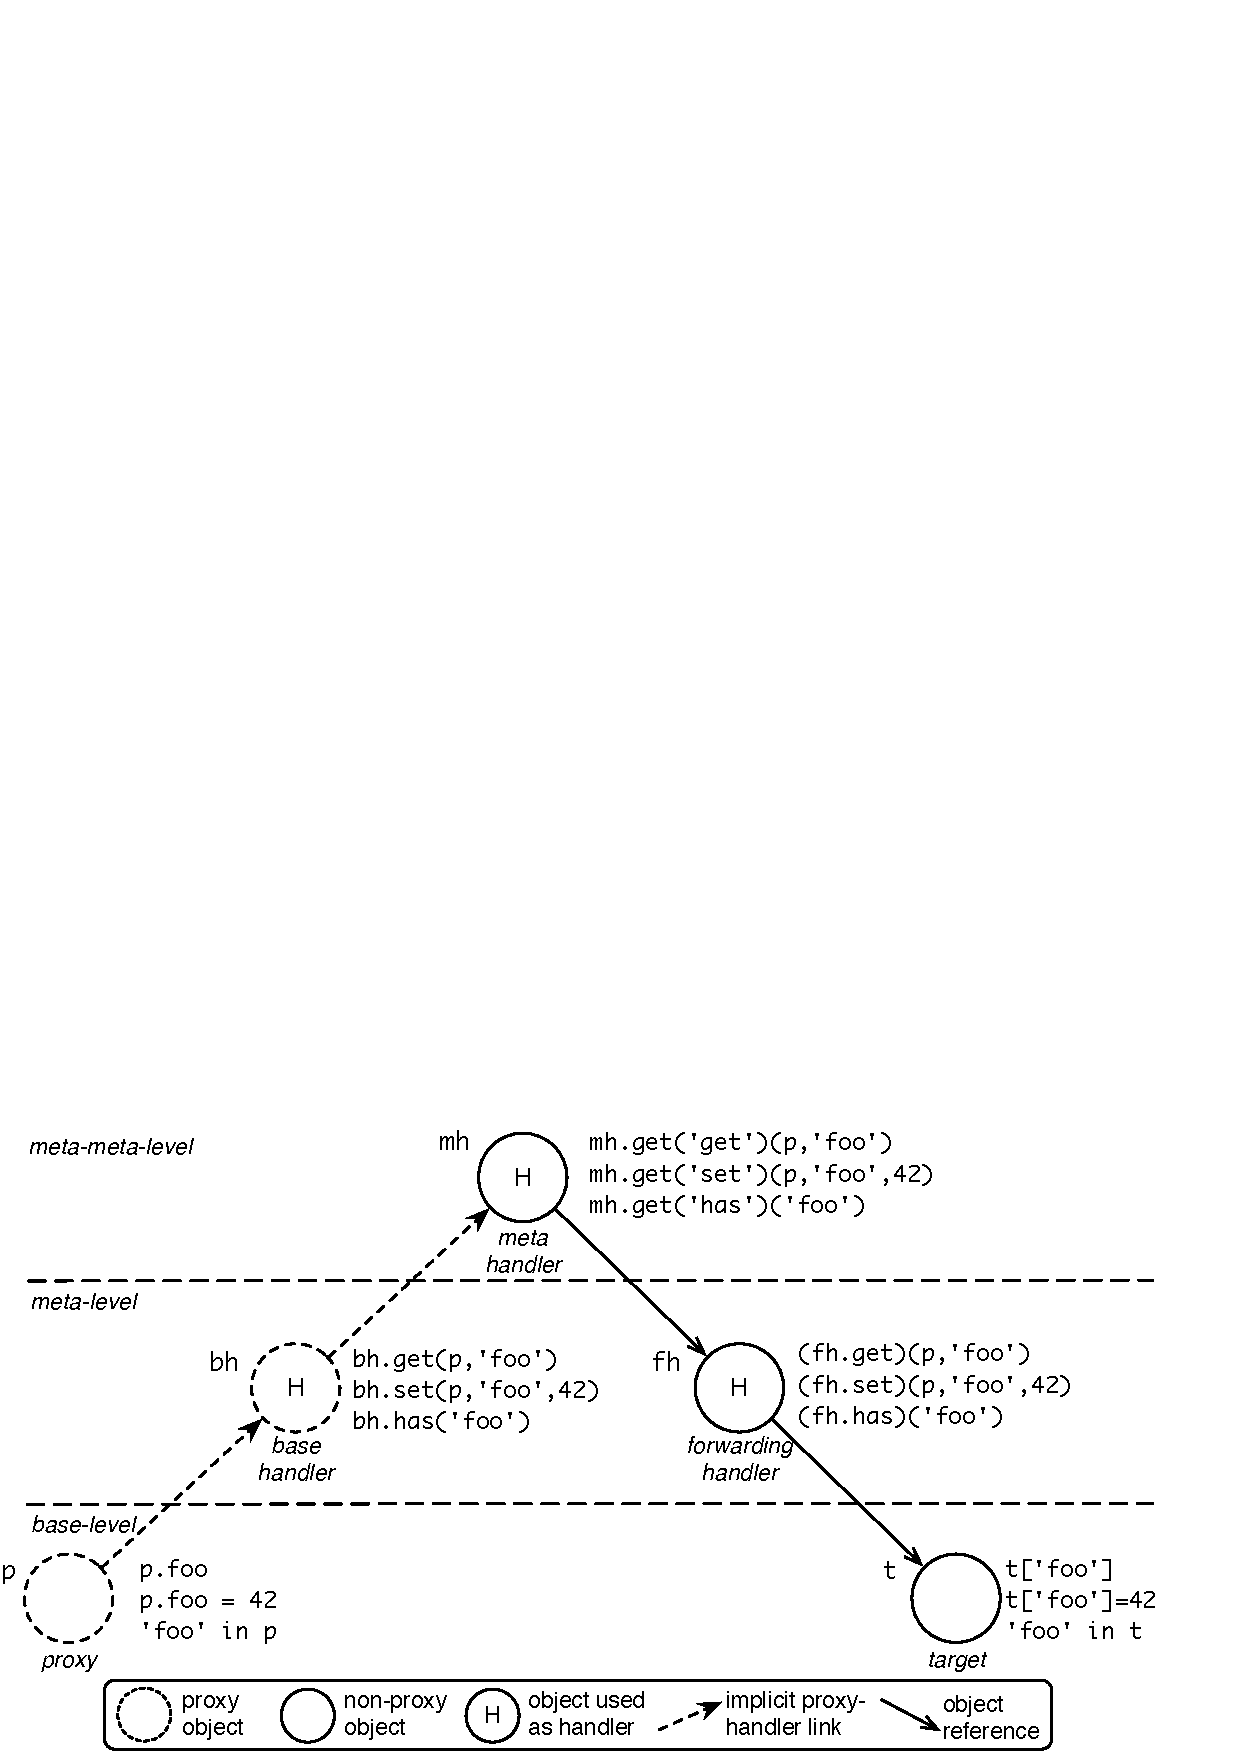
\includegraphics[width=1.0\columnwidth]{MetaLevelShifting.png}
  \caption{Meta-level shift using a proxy as a handler}
  \label{fig:shift}
\end{figure}

Figure~\ref{fig:shift} depicts how meta-level shifting works. Note that the base handler is both a handler and itself a proxy. Note also how all operations performed on \texttt{p} are intercepted by \texttt{mh}'s \texttt{get} trap.

Another way to explain why this funneling works is as follows. At the base-level, there is an assortment of operations that are performed on Javascript objects as computation progresses (e.g. property lookup, access, assignment, enumeration, \ldots). At the meta-level (that is: in the intercession API), all of these operations are reified uniformly as method invocations on handlers. Therefore, at the meta-level, the only operation performed on meta-level objects (base-level handlers) is property access, and meta-meta-level objects (meta-level handlers) only need to handle this single operation in their protocol.

If one shifts an extra level upwards to funnel all operations through a single trap of a meta-level handler, one must also shift an extra level downwards if these operations must eventually be applied to a base-level object. This can be accomplished by having the meta-level handler forward the operations to a generic forwarding handler. The forwarding handler essentially translates meta-level operations back into base-level operations on a target object.

Naturally, one can apply this trick of shifting meta-levels at the meta-meta-level recursively. The API allows an arbitrary number of such meta-level shifts. This brings up the question of infinite meta-regress. Such an infinite regress is avoided as long as a proxy handler is eventually implemented as a concrete Javascript object, rather than as yet another proxy.

% Design Principle: handlers can be proxies themselves
% Design Principle: express all meta-level computation (interaction with the handler)
% using a single primitive such that shifting two levels requires intercession of only one operation
To summarize, this section reveals two important design principles of proxy-based intercession APIs:

\textbf{Meta-level shifting:} a proxy-based intercession API supports shifting to a new meta-level by implementing a handler as a proxy.

\textbf{Meta-level funneling:} the interaction between a proxy and its handler determines the API of the meta-meta-level. If the proxy only invokes the handler's traps, then the meta-meta-level API collapses to a single trap through which all meta-level operations are funneled.

Meta-level funneling is demonstrated in Section~\ref{sub:revoker}.

%\textbf{Funneling trap:} the trap through which all meta-level operations can be funneled, either directly or using mechanisms such as meta-level funneling.

%For Javascript proxies, \texttt{get} is the funneling trap.

\subsection{Selective Interception}
\label{sub:selective}
% tradeoff between what to intercess and what to fix upfront

A proxy-based intercession API introduces a tradeoff between what operations can be intercepted by proxy handlers on the one hand, versus what operations have a reliable outcome from the language runtime and the programmer's point of view. We already briefly touched upon this issue in Section~\ref{sub:immutability} when discussing how proxies interact with operations that make objects non-extensible, sealed or frozen. As we have discussed, the \texttt{fix} trap enables a proxy handler to dynamically decide whether or not to commit to a fixed representation.

% commit to identity upfront (possible because we don't intercess equality)
Some operations may be so critical that we don't want proxies to influence their outcome. One such operation is testing for equality. In Javascript, the expression \texttt{a === b} determines whether \texttt{a} and \texttt{b} refer to identical objects. The \texttt{===} operator comes with an entire list of guarantees that are implicitly taken for granted by programmers. For example, \texttt{===} is commutative, transitive, symmetric and deterministic (it always reports the same answer given the same arguments). Furthermore, testing \texttt{a} and \texttt{b} for equality should not grant \texttt{a} access to \texttt{b} or vice versa. For all these reasons, we decided not to enable proxy handlers to trap \texttt{===}. Proxies cannot influence the outcome of this operation.

As in the case of \texttt{===}, the fact that an operation should be deterministic is a requirement for many operations. To uphold determinism, the operation should not be delegated to a proxy handler. However, just because an operation should have a deterministic result does not mean that it cannot be reliably intercepted. When an operation requires a deterministic, stable result, this result can be provided once to the proxy when it is created. There are two concrete examples of this in our intercession API.

The first example is that proxies must commit to their prototype upfront. Recall from section~\ref{sec:proxies_for_javascript} that the second argument to \texttt{Proxy.create} denotes the proxy's prototype. This has two important effects: the first is that ECMAScript's built-in operation \texttt{Object.getPrototypeOf} remains deterministic, even when applied to a proxy. The second is that proxies cannot influence \texttt{instanceof} when they are used as the left-hand operand: to determine whether \texttt{proxy instanceof Foo} is true, the implementation need only look at the prototype of \texttt{proxy}, which using our API it can do without consulting the proxy.

The second example is that proxies have to decide upfront whether they will proxy a plain object or a function object. By requiring proxies to commit to representing either an object or a function at proxy creation time, the language runtime is able to uphold important invariants that it would have to forfeit if it would have to consult the \texttt{handler}. For example the expression \texttt{typeof o} should evaluate to \texttt{"function"} if \texttt{o} is a function, and to \texttt{"object"} otherwise. Also, functions always inherit from \texttt{Function.prototype}. The distinction between object and function proxies allows our API to enforce these invariants.

Another aspect to take into account when deciding whether or not a certain operation can be intercepted by a proxy is the fact that it may lead to arbitrary code being run in places where the language runtime or the programmer did not expect this to. For example, without our intercession API, the expression \texttt{name in obj} does not trigger Javascript code. Since \texttt{in} is a primitive operation, the evaluation of this expression occurs entirely within the language runtime, without it ever having to run non-native code. Proxies may change these assumptions.

In our particular case, proxies enable non-native code to run while evaluating the \texttt{in} operator, the \texttt{delete} operator and \texttt{for-in} loops, yet they preserve the integrity of \texttt{===} and \texttt{typeof}. It's hard to make general claims about what operations should generally be interceptable and which should not. It is a design decision that depends on the particulars of the system at hand. The point that we want to make is that it's important to recognize that such a tradeoff exists. This brings us to the following design principle:

\textbf{Selective interception:} determine what properties of an object should be to committed to upfront. If these properties are required to be stable but may be configurable, turn them into parameters of the proxy constructor rather than retrieving them via a handler trap.

\subsection{Fundamental versus derived traps}
\label{sub:fundamental_vs_derived_traps}

As shown in Table~\ref{tab:operations}, our handler API defines 12 traps in total, each intercepting a different Javascript operation applied to a proxy. However, some traps can be expressed in terms of the semantics of other traps (i.e. the semantics of the operation which they intercept is subsumed by the semantics of some other operation). We refer to such traps as \emph{derived} traps, since their implementation may be derived from other, more \emph{fundamental} traps.

\subsubsection{Efficiency: the case for derived traps}

Our handler API is comprised of 7 fundamental traps and 5 derived traps. If 7 traps are sufficient to faithfully emulate an object, why define 12 of them? The reason is efficiency: implementing a derived trap directly may be more efficient than using its default implementation based on the corresponding fundamental trap. In our particular design, as a rule of thumb, we introduced derived traps only if their implementation could intercept the operation with fewer allocations than the corresponding implementation based on the fundamental trap.

As a concrete example, consider the expression \texttt{name in obj}. The \texttt{in} operator returns a boolean indicating whether \texttt{obj} defines or inherits a property named \texttt{name}. If \texttt{obj} is a proxy, this operation triggers the handler's \texttt{has(name)} trap, which should return a boolean. \texttt{has} is a derived trap: its semantics can be directly derived from the fundamental trap \texttt{getPropertyDescriptor} which, given a property name, returns either a property descriptor for a property corresponding to that name if it exists, or returns \texttt{undefined} otherwise. Clearly, \texttt{has} could have just been defined implicitly as:

\begin{lstlisting}[language=javascript]
has: function(name) {
  return this.getPropertyDescriptor(name) !== undefined;
}
\end{lstlisting}

The downside of this implementation is that \texttt{getPropertyDescriptor} must needlessly allocate a property descriptor object if the named property exists. A custom implementation of \texttt{has} can often avoid this allocation.

%Note that it's possible to create an ``abstract'' prototype object that implements all derived traps in terms of the more fundamental traps. Since a handler is just a regular object, it can delegate to this abstract prototype to inherit the default derived traps, provided it implements the fundamental traps.

While defining the intercession API, we found that there is another force at play that can prevent designers from introducing a derived trap, even if it were more efficient.

\subsubsection{Consistency: the case against derived traps}

One reason not to introduce a derived trap, even in the face of improved efficiency, is that introducing the distinction may break language invariants that may surprise the language runtime and programmers.

Once the API provides a proxy handler with both a fundamental and a derived trap, there is no guarantee that a proxy handler will effectively make sure that the derived trap is indeed semantically equivalent to the canonical derived implementation. For example, if a proxy handler is given the option to override both the \texttt{has} and the \texttt{getPropertyDescriptor} traps, it is not enforced that these traps return mutually consistent results. Without proxies, the programmer can count on the invariant that \texttt{name in obj} is equivalent to \texttt{Object.getPropertyDescriptor(obj, name) !== undefined}. If \texttt{obj} is a proxy, this invariant is no longer guaranteed: \texttt{has} could return true and \texttt{getPropertyDescriptor} could nevertheless return \texttt{undefined}.

For proxies, both the language runtime and programmers can no longer count on such invariants being upheld, although a ``correct'' handler should attempt to uphold them. Even if the handler implementor does not intend to violate the invariants, the distinction between fundamental and derived traps nevertheless introduces a maintenance cost: if either of the two traps is changed or gets overridden in a delegating object, the other trap should be changed or overridden in a compatible way.

The requirement of mutual consistency between operations is an opposing force in the decision of whether or not to introduce a derived trap for a certain operation. Whether the benefits of efficiency outweigh the mutual consistency of operations is, again, based on the particulars of the system and there is no general answer.

\textbf{Fundamental versus Derived Traps:} an intercession API faces a tradeoff between defining a minimal API consisting only of fundamental traps versus defining a more complex API that introduces derived traps. Derived traps may be more efficient, but may break invariants that hold between the operations corresponding to the fundamental and the derived trap.

%One interesting case where mutual consistency outweighed efficiency gain was the decision not to introduce a derived trap to intercept method invocations. In Javascript, a method call expression \texttt{obj.m(1,2,3)} is evaluated by looking up the property \texttt{m} in \texttt{obj}, and then applying the resulting value to the arguments, as if by executing \texttt{var f = obj.m; f.apply(obj, [1,2,3])}.

%In a first design iteration, we defined a separate trap for method invocations: the expression \texttt{proxy.m(1,2,3)} would call \texttt{handler.invoke(obj,'m',[1,2,3])} where \texttt{handler} is \texttt{proxy}'s handler. The expression \texttt{proxy.m} calls \texttt{handler.get(proxy, 'm')}. Clearly, given the invariant sketched in the previous paragraph, \texttt{invoke} is a derived trap corresponding to the more fundamental \texttt{get} trap. Its canonical derived implementation would be:

%\begin{lstlisting}[language=javascript]
%invoke: function(rcvr, name, args) {
%  return this.get(rcvr, name).apply(rcvr, args);
%}
%\end{lstlisting}

%\texttt{invoke} is a useful derived trap because in some cases it can avoid the allocation of a function. Say a proxy wants to virtualize some non-object resource as an object. Say this resource has a property \texttt{foo} that should behave like a method. Part of the proxy handler's traps could be implemented as follows:

%\begin{lstlisting}[language=javascript]
%get: function(rcvr, name) {
%  if (name === 'foo') {
%    return function() {
%      // this is a variable-argument function
%      // that handles proxy.foo(arguments)
%    } 
%  } else ...
%},
%invoke: function(rcvr, name, args) {
%  if (name === 'foo') {
%    // handle proxy.foo(args)
%  } else ...
%}
%\end{lstlisting}

%Since the \texttt{get} trap does not get direct access to the arguments of a call, it has to return a function to curry over the arguments of the invocation. The \texttt{invoke} trap does not need to allocate this intermediate function. Eventually, we dropped the \texttt{invoke} trap because the invariant that it can break is so deeply rooted in the understanding of Javascript's method invocation semantics.

\subsection{Handler Encapsulation}
\label{sub:meta_level_encapsulation}

A Proxy-based intercession API encapsulates its handler if, given a reference to a proxy, one cannot gain direct access to the proxy's handler. For our proxy API, this is the case. If a handler can be encapsulated behind its proxy, the handler can ensure that its traps can only ever be invoked by manipulating its corresponding proxy.

If the handler explicitly wants to be accessible from its proxy, it can cater to such access itself without violating stratification. The handler could register the association between its proxy and itself in a registry. Objects with access to this registry and to the proxy can then look up the handler, using the proxy as a key. Such a registry plays a similar role in our architecture as mirror factories in a mirror-based architecture (see Section~\ref{sub:mirrors}).

%If access to a proxy's handler is required, it is fairly straightforward for the proxy creator to provide such access. For example, the proxy creator could define its own proxy factory:

%\begin{lstlisting}[language=javascript]
%function MyProxyFactory() {
%  var proxies = new EphemeronTable();
%  return {
%    create: function(handler, proto) {
%      var proxy = Proxy.create(handler, proto);
%      proxies.put(proxy, handler);
%      return proxy;
%   },
%    handlerOf: function(proxy) {
%      return proxies.get(proxy);
%    }
%  };
%}
%\end{lstlisting}

%If a proxy \texttt{p} was generated using such a proxy factory \texttt{pf}, objects are able to retrieve the proxy's handler by invoking \texttt{pf.handlerOf(p)}.

%An \texttt{EphemeronTable} is almost identical to a non-enumerable weak-key hashtable, but it avoids a crucial memory leak when cyclic dependencies exist between the keys and the values stored in the table. It is based on Smalltalk's Ephemerons~\cite{et_paper} and is a new abstraction proposed for inclusion in ES-Harmony~\cite{miller10et}. Using ephemeron tables, it's fairly straightforward to link a proxy to its handler without actually having to manipulate the proxy.

\subsection{Uniform Intercession}
\label{sub:uniform_intercession}

Eugster~\cite{eugster06uniform} introduces the term \emph{uniform proxies} to denote an object model in which objects of all types can be proxified. More generally, we state that an intercession API is uniform if it enables the creation of proxies for all possible types of values in the language. Javascript proxies do not support uniform intercession, since they are only able to proxy for objects (object proxies) or functions (function proxies). Primitive values cannot be proxified.

The advantage of having a uniform intercession API is that it does not restrict programmers to use only language values that can be proxied. Conversely, it enables meta-programmers to potentially use the intercession API on more base-level objects.

%could be another important design principle: whether or not to fully virtualize an API
%A method is defined on \texttt{Proxy} to distinguish trapping proxies from regular objects or fixed proxies:
%\texttt{Proxy.isTrapping(anObject)} returns \texttt{true} if and only if \texttt{anObject} is a proxy and is in trapping mode. This is the single, reliable way of testing whether an object is a trapping proxy or not. Note that a proxy cannot influence the outcome of this method. Once a proxy is fixed, it is in all ways simply a normal object, with no built-in way to detect that it had ever been a trapping proxy.

\section{Access Control Wrappers}
\label{sec:examples}

We now show how to apply our Proxy API to implement generic wrappers for access control purposes.

\subsection{Revocable Object References}
\label{sub:revoker}

Say an object \texttt{Alice} wants to hand out to \texttt{Bob} a reference to \texttt{Carol}. \texttt{Carol} could represent a precious resource, and for that reason \texttt{Alice} may want to limit the lifetime of the reference it hands out to \texttt{Bob}. In other words, \texttt{Alice} wants to have the ability to revoke \texttt{Bob}'s access to \texttt{Carol}.

One can implement this pattern of access control by wrapping \texttt{Carol} in a forwarder that can be made to stop forwarding. Such a forwarder is also known as a \emph{caretaker}~\cite{redell74naming}. Without proxies, the programmer is forced to write a distinct caretaker for each kind of object that should be wrapped. Proxies enable the programmer to abstract from the details of the wrapped object's protocol and instead write a \emph{generic} caretaker\footnote{For brevity, we left out the case in which \texttt{target} is a function, requiring the caretaker to be a function proxy.}:

\begin{lstlisting}[language=javascript]
function makeRevocableRef(target) {
  var enabled = true;
  return Object.freeze({
    caretaker: Proxy.create({
      get: function(rcvr, name) {
        if (!enabled) { throw new Error("revoked"); }
        return target[name];
      },
      has: function(name) {
        if (!enabled) { throw new Error("revoked"); }
        return name in target;      
      },
      // ... and so on for all other traps
    }, Object.getPrototypeOf(target)),
    revoker: Object.freeze({
      revoke: function() { enabled = false; }
    })
  });
}
\end{lstlisting}

Given this abstraction, \texttt{Alice} can now wrap \texttt{Carol} in a revokable reference, pass the caretaker to \texttt{Bob}, and hold on to the revoker such that access can later be revoked.

The caretaker is a proxy whose handler is very similar to the generic forwarder defined in Section~\ref{sec:proxies_for_javascript} except that it explicitly checks the \texttt{enabled} flag before forwarding. As noted in Section~\ref{sub:doublelifting}, this is a pattern that can itself be abstracted by shifting meta-levels once more. If the caretaker's handler is itself a proxy, the meta-level handler can funnel all meta-level operations through a single \texttt{get} trap:

\begin{lstlisting}[language=javascript]
function makeRevocableRef(target) {
  var enabled = true;
  var fwdHandler = makeForwardingHandler(target);
  var baseHandler = Proxy.create({
    get: function(rcvr, name) {
      if (!enabled) { throw new Error("revoked"); }
      return fwdHandler[name];
    }
  });
  return Object.freeze({
    caretaker: Proxy.create(baseHandler,Object.getPrototypeOf(target)),
    revoker: Object.freeze({
      revoke: function() { enabled = false; }
    })
  });
}
\end{lstlisting}

A limitation of the above caretaker abstraction is that objects exchanged via the caretaker are themselves not recursively wrapped in a revocable reference. For example, if \texttt{Carol} defines a method that returns \texttt{this}, an unwrapped reference may be exposed to \texttt{Bob}, circumventing the caretaker. This is an instance of the \emph{two-body problem}~\cite{eugster06uniform}, the fact that wrappers may be ``leaky'' because the wrapping proxy and the wrapped object are distinct entities. The abstraction discussed in the following section addresses this issue.

%Note that the two-body problem is \emph{not} related to the fact that a proxy and its \emph{handler} are distinct. It is a limitation inherent to using proxies as generic wrappers, not to using separate proxy handlers to achieve stratification.

%\subsection{The Two-body Problem}

%Eugster~\cite{eugster06uniform} calls attention to a limitation of the proxy approach to generic wrappers, which he coins the \emph{two-body problem}: the fact that the proxy and the wrapped object are distinct entities. The problem is that the proxy abstraction may ``leak'' the wrapped object, in two ways:
%\begin{enumerate}
%  \item If the proxy handler simply forwards a method call to the wrapped target object, and the target object subsequently performs a self-send, the proxy cannot intercept that method call anymore.
%  \item If the wrapped object returns a reference to itself, it may expose a direct (unwrapped) reference to itself to its clients. It is the task of the proxy handler to detect this and instead return a reference to the proxy.
%\end{enumerate}

%Problem 1 can be solved by having the proxy handler \emph{delegate} the request rather than \emph{forward} the request. Delegation, unlike normal method invocation, does not modify the receiver of the invocation~\cite{lieberman86prototypical}. In Javascript, proxy handlers can easily encode delegation by rebinding a wrapped function's \texttt{this} pseudovariable to the proxy instead.

%If one factors out the specifics of revocation, the membrane abstraction from Section~\ref{sub:membranes} is in fact a general-purpose solution to problem 2. However, as mentioned previously in that section, for a workable membrane to be practically useful, it is crucial that the membrane uphold object-equality on both sides of the membrane (i.e. two proxies are \texttt{===} if and only if their wrapped objects are). Ephemeron tables~\cite{miller10et} are the key abstraction that enable this without introducing memory leaks.

\subsection{Membranes}
\label{sub:membranes}
% es-lab's compartments building on membranes

A membrane is an extension of a caretaker that transitively imposes revocability on all references exchanged via the membrane~\cite{miller06robust}. In the following implementation, we make use of meta-level funneling once more to centralize the access control in a single trap:

\begin{lstlisting}[language=javascript]
function makeMembrane(initTarget) {
  var enabled = true;
  function wrapFunction(f) {
    return function() { // variable-argument function
      if (!enabled) {throw new Error("revoked");}
      try {
        return wrap(f.apply(wrap(this), toArray(arguments).map(wrap)));
      } catch (e) { throw wrap(e); } 
    }
  }
  function wrap(target) {
    //primitives provide irrevocable knowledge, no need to wrap them
    if (isPrimitive(target)) { return target; }
    var fwdHandler = makeForwardingHandler(target);
    var baseHandler = Proxy.create({
      get: function(rcvr, name) {
        return wrapFunction(fwdHandler[name]);
      }
    });
    
    if (typeof target === "function") {
      var wrappedF = wrapFunction(target);
      return Proxy.createFunction(baseHandler, wrappedF);
    } else {
      return Proxy.create(baseHandler,
                          wrap(Object.getPrototypeOf(target)));
    }
  }
  return Object.freeze({
    wrapper: wrap(initTarget),
    revoker: Object.freeze({
      revoke: function() { enabled = false; }
    })
  });
}
\end{lstlisting}

A membrane consists of one or more wrappers. Every such wrapper is created by a call to the \texttt{wrap} function. Note that all wrappers belonging to the same membrane share a single \texttt{enabled} variable. Assigning the variable to \texttt{false} revokes all of the membrane's wrappers simultaneously.

Recall that this example makes use of meta-level funneling. The \texttt{baseHandler} is itself a proxy with a handler. This handler need only implement a \texttt{get} trap that returns a meta-level trap (a function) that will immediately be invoked. To be able to wrap the arguments of these invocations, the \texttt{get} trap returns a wrapped version of the default forwarding trap contained in the \texttt{fwdHandler}.

If the object to be wrapped is a function (or a method, because Javascript methods are just functions), a function proxy is returned whose call trap is a wrapped version of the function, as defined by \texttt{wrapFunction}. The variable-argument function\footnote{In Javascript, \texttt{arguments} is an object that contains all arguments passed to a function. It is used to write variable-argument functions, and it is customary to convert this object into a proper array first.} returned by \texttt{wrapFunction} performs the actual wrapping of values that cross the membrane: arguments to methods cross the membrane in one direction, returned values or thrown exceptions in the other direction.

The membrane abstraction in Javascript enables innovative new ways of composing code from untrusted third parties on a single web page (so-called ``mash-ups''). By loading the untrusted code using a membrane-wrapped \texttt{eval} function, it becomes possible to isolate scripts from one another and from their container page.

\paragraph{Identity-preserving Membranes} One problem with the above membrane abstraction is that it fails to uphold object identity across both sides of the membrane. If an object \texttt{o} is passed through the same membrane twice, an object on the other side of the membrane will receive two distinct wrappers \texttt{w1} and \texttt{w2}, such that \texttt{w1~!==~w2}, even though both wrap an identical object. Likewise, passing \texttt{w1} or \texttt{w2} back through the membrane does not unwrap them but rather wraps them again. These limitations can be addressed by having the membrane maintain two maps. The first maps objects to their wrappers, such that only one canonical wrapper is created per object. The second maps wrappers back to the objects they wrap, allowing these objects to be unwrapped when they cross the membrane in the other direction.

Unfortunately, implementing these maps in Javascript is impossible without introducing memory leaks. Ephemeron tables are a proposed language feature for the upcoming ECMAScript standard that address this issue~\cite{miller10et}. An ephemeron table is almost identical to a non-enumerable weak-key identity hashtable, but it avoids a crucial memory leak when cyclic dependencies exist between the keys and the values stored in the table.
%It is based on Smalltalk's Ephemeron pairs~\cite{et_paper}.
%A membrane around an SES \texttt{eval}\footnote{Ref to \texttt{es-lab} project for SES and Securable ES5.} creates a compartment in which one can run potentially malicious code, confident that the resulting potentially malicious objects can interact with the world outside this compartment only as permitted by the objects you provide them. Once the compartment is revoked, all their connectivity with its outside environment is severed, rendering it powerless.

%\subsection{Script Compartments}

%In a capability-secure subset of ECMAScript~\cite{ses}, if a membrane is used to wrap the \texttt{eval} function, it becomes possible to write mash-ups combining mutually suspicious pieces of code that can be isolated from one another and the container page:

%\begin{lstlisting}[language=javascript]
%var compartment = makeMembrane(eval);
%var safeEval = compartment.wrapper;
%var badCode = //load potentially malicious code
%var result = safeEval(badCode);
%//use result
%compartment.revoker.revoke();
%//contents of compartment gone and collectible
%\end{lstlisting}

%A membrane around an SES \texttt{eval}\footnote{Ref to \texttt{es-lab} project for SES and Securable ES5.} creates a compartment in which one can run potentially malicious code, confident that the resulting potentially malicious objects can interact with the world outside this compartment only as permitted by the objects you provide them. Once the compartment is revoked, all their connectivity with its outside environment is severed, rendering it powerless.

\section{Implementation}
\label{sub:benchmarks}

Andreas Gal has implemented a prototype of our proposed Proxy API for Javascript as an extension of Tracemonkey. Tracemonkey is an extension of Spidermonkey, Mozilla's Javascript engine, that employs trace trees for aggressive optimization~\cite{gal06efficient}\footnote{Progress on this extension can be tracked at \url{https://bugzilla.mozilla.org/show_bug.cgi?id=546590}}.

We used the prototype implementation to get an initial idea of the overhead of our Proxy API. To this end, we performed the following micro-benchmark: first, we measured the runtime of the various operations applied to regular objects in regular Tracemonkey, without any Proxy API extensions. Next, we measured the runtime of the same operations, this time on regular, \emph{non-proxy} objects in the Tracemonkey extension with support for proxies. Finally, we measured the runtime of the operations on a \emph{proxy} object whose handler is the default forwarding handler introduced in Section~\ref{sec:proxies_for_javascript}.

\begin{table}
  \begin{center}
  \begin{tabular}{r|r|r|r|r|r}
    %\hline
              & \multicolumn{1}{|c|}{Proxies} & \multicolumn{4}{|c}{Proxies}\\
              & \multicolumn{1}{|c|}{Disabled} & \multicolumn{4}{|c}{Enabled}\\
    \hline
           &   & \multicolumn{2}{|c|}{(non-proxy)} & \multicolumn{2}{|c}{(proxy)}\\
           \cline{3-6}
 Operation & \multicolumn{1}{|c|}{$a$} & \multicolumn{1}{|c|}{$b$} & \multicolumn{1}{|c|}{$c=b/a$} & \multicolumn{1}{|c|}{$d$} & \multicolumn{1}{|c}{$e=d/b$}\\
    \hline
    typeof     & ~.38 $\mu$\emph{s} & .39 & \textbf{1.02} & .39 & \textbf{1.00}\\
    instanceof & ~.49 $\mu$\emph{s} & .51 & \textbf{1.04} & .52 & \textbf{1.01}\\
    call       & ~.47 $\mu$\emph{s} & .47 & \textbf{1.00} & .61 & \textbf{1.29}\\
    delete     & ~.42 $\mu$\emph{s} & .42 & \textbf{1.00} & .71 & \textbf{1.69}\\
    has        & ~.41 $\mu$\emph{s} & .41 & \textbf{1.00} & .73 & \textbf{1.78}\\
    set        & ~.40 $\mu$\emph{s} & .41 & \textbf{1.02} & .74 & \textbf{1.80}\\
    get        & ~.38 $\mu$\emph{s} & .39 & \textbf{1.03} & .73 & \textbf{1.87}\\
    enumerate  & 1.58$\mu$\emph{s} & 1.58 & \textbf{1.00} & 4.0 & \textbf{2.53}\\
   % \hline
  \end{tabular}
  \end{center}
  \caption{Micro-benchmarks measuring overhead of the Proxy API (c) and of a proxy wrapper (e).}
  \label{tab:benchmarks}
\end{table}

The results are shown in Table~\ref{tab:benchmarks} for a subset of the operations. They were obtained on a MacPro Dual-core Intel Xeon (2.66Ghz) with 4GB Memory, running Mac OS X 10.5.8, using the following version of Tracemonkey: \url{http://hg.mozilla.org/tracemonkey/file/eba4f78cdca4}. Runtimes shown are an average over multiple runs.

The results in column (c) show that the addition of proxies in the virtual machine introduces no significant overhead for non-proxy objects. Hence, proxies only introduce a performance penalty when they are needed.

The results in column (e) show the overhead of using proxies to implement generic wrappers. Traps are ordered from least to most overhead. Our results confirm that operations like \texttt{typeof} and \texttt{instanceof} that do not consult the handler introduce no overhead. The overhead of intercepting the other operations, save enumeration, is less than a factor of 2. The overhead comes from the additional invocation of the handler method. Presumably, the \texttt{get} and \texttt{set} traps introduce the most overhead because they are the most optimized for non-proxy objects. Enumeration is the only operation that is more than twice as slow when applied to proxies. This is because enumeration must now proceed by iterating over a user-created array returned by the \texttt{enumerate} trap, rather than using the built-in iteration algorithm.

\section{Related Work}

\subsection{OO Intercession APIs: a comparison}
\label{sub:survey}

In this section we summarize a variety of message-based, object-oriented intercession APIs. We discuss whether and how each of them upholds the design principles put forth in Section~\ref{sec:proxies_for_javascript}. We do not claim that our survey is exhaustive, but we believe the most representative intercession APIs are covered. We briefly discuss the surveyed mechanisms and then summarize which of our design principles they uphold in Table~\ref{tab:related_work}.

\textbf{Java} The Java 1.3 \texttt{java.lang.reflect.Proxy} API is a major precedent to our Javascript proxy API. Java's dynamic proxies can be used to intercept invocations on instances of interface types:

\begin{lstlisting}[language=java]
InvocationHandler h = new InvocationHandler() {
  Object invoke(Object pxy, Method m, Object[] args) {...}
};
Foo proxy = (Foo) Proxy.newProxyInstance(
  aClassloader, new Class[] { Foo.class }, h);
\end{lstlisting}

Here, \texttt{proxy} implements the \texttt{Foo} interface. \texttt{h} is an object that implements a single \texttt{invoke} method. All method invocations on \texttt{proxy} are reified by calling the \texttt{h.invoke} method, passing along a description of the invoked method and the arguments of the call.

The main difference between Java proxies and Javascript proxies is that Java proxies can only intercept method invocation. There are no other meta-level operations to trap. For instance, since interfaces cannot declare fields, proxies do not need to intercept field access.

The Java Proxy API is non-uniform: proxies can only be constructed for interface types, not class types. As a result, proxies cannot be used in any situation where code is typed using class types rather than interface types, limiting their general applicability. Eugster~\cite{eugster06uniform} describes how to extend the Java Proxy API to work uniformly with instances of non-interface classes. Next to the usual \texttt{InvocationHandler}, proxies for class types have an additional \texttt{AccessHandler} to trap field access.

%Implementation-wise, another important difference is that Java proxies can be supported by a JVM without the need for a special ``proxy'' object type. A description of the proxy (and all of its methods) can be generated from the given interfaces and subsequently instantiated as a normal object (whose class just happens to be synthesized at runtime).

%Mirages in AmbientTalk: adds intercession to a Mirror API
\textbf{AmbientTalk} The design of Javascript proxies was influenced by AmbientTalk \emph{mirages}~\cite{mostinckx07behavioral}. AmbientTalk is a distributed dynamic language, with a mirror-based meta-level API. AmbientTalk enables intercession through mirages, which are proxy-like objects controlled explicitly by a separate mirror object:

\begin{lstlisting}[]
def mirage := object: {...} mirroredBy: (mirror: {
  def invoke(receiver, message) { ... };
  def addSlot(slot) { ... };
  def removeSlot(slot) { ... };
  ...
});
\end{lstlisting}

The mirror is to the mirage what the proxy handler is to a Javascript proxy. Like Javascript proxy handlers, mirrors define an extensive set of traps, enabling near-complete control over the mirage.

\textbf{E} E is a secure, distributed dynamic language~\cite{miller05concurrency}. In E, everything is an object, but there are two kinds of object references: \emph{near} and \emph{eventual} references. Similarly, there are two message passing operators: immediate call (\texttt{o.m()}, a synchronous method invocation) and eventual send (\texttt{o<-m()}, an asynchronous message send). Both operations are allowed on near references, but eventual references carry only asynchronous messages. Because of this distinction, E has two separate intercession APIs: one for objects and one for references.

E has a proxy-based API to represent user-defined eventual references~\cite{eproxies}:

\begin{lstlisting}[]
def handler {
  to handleSend(verb :String, args :List) {...}
  to handleSendOnly(verb :String, args :List) {...}
  to handleOptSealedDispatch(brand) {...}
}
def proxy := makeProxy(handler, slot, state);
\end{lstlisting}

This API is very similar to the one for Javascript proxies. The proxy represents an eventual reference, and any asynchronous send \texttt{proxy<-m()} either triggers the handler's \texttt{handleSend} or \texttt{handleSendOnly} trap, depending on whether the sender expects a return value.

The \texttt{handleOptSealedDispatch} trap is part of E's trademarking system and is beyond the scope of this paper. The \texttt{slot} argument to \texttt{makeProxy} can be used to turn the proxy reference into an actual, so-called \emph{resolved} reference. Once a reference is resolved, the proxy is bypassed and the handler no longer consulted. It fulfills a role similar to the \texttt{fix} trap described in Section~\ref{sub:immutability}. The \texttt{state} argument to \texttt{makeProxy} determines the state of the reference. The details are outside the scope of this paper, but note that this allows the eventual reference proxy to determine its state without consulting the handler, similar to how Javascript proxies can determine their prototype without consulting the handler.

E has a distinct intercession API for objects. A \emph{non-methodical object} is an empty object with no methods. Instead, its implementation consists of a single \texttt{match} clause that encodes an explicit message dispatch:

\begin{lstlisting}
def obj match [verb, args] {
  # handle the message generically
}
\end{lstlisting}

The variable \texttt{obj} is bound to a new object whose dispatch logic, if any, is explicitly encoded in the \texttt{match} clause. An immediate call \texttt{obj.m(x)} will trigger this clause, binding \texttt{verb} to \texttt{"m"} and \texttt{args} to a list \texttt{[x]}.

Finally, it is worth noting that AmbientTalk inherits from E the distinction between near and eventual references and the distinction between immediate call and eventual send. Unlike E, AmbientTalk has only one intercession API (mirages), but a mirage can represent \emph{both} objects and eventual references, depending on how the handler implements its traps (immediate calls and eventual sends each trigger a separate trap).

\textbf{Smalltalk} Smalltalk-80 popularized generic message dispatch via its \texttt{doesNotUnderstand:} mechanism. Briefly, if standard method lookup does not find a method corresponding to a message, the Smalltalk VM instead sends the message \texttt{doesNotUnderstand: msg} to the original receiver object. Here, \texttt{msg} is an object containing the message's selector and arguments. The default behavior of this method, inherited from \texttt{Object} is to throw an exception.

The \texttt{doesNotUnderstand:} trap is not stratified. It occupies the same namespace as plain application-level methods. This lack of stratification did lead Smalltalk programmers to look for alternative interception mechanisms. Foote and Johnson describe a particular extension to ParcPlace Smalltalk called a \emph{dispatching class}: ``Whenever an object belonging to a class designated as a dispatching class (using a bit in the class object's header) is sent a message, that object is instead sent \texttt{dispatchMessage: aMessage}.''~\cite{foote89reflective}. Instances of dispatching classes are effectively proxies, the \texttt{dispatchMessage:} method acting as the sole trap of an implicit handler.

Ducasse~\cite{ducasse99evaluatingmessage} gives an overview of the various message passing control techniques in Smalltalk. He concludes that \texttt{doesNotUnderstand:} is not always the most appropriate mechanism. Rather, he stresses the usefulness of \emph{method wrappers}. This approach was elaborated by Brant \emph{et. al}~\cite{brant98wrappers}. In this approach, rather than changing the method \emph{lookup}, the method \emph{objects} returned by the lookup algorithm are modified. This is possible because Smalltalk methods and method dictionaries are accessible from within the language. The method wrapper approach is in many ways similar to CLOS method combinations, enabling before/after/around augmentation of existing methods. As their name suggests, they are great for wrapping existing methods, but they seem less suitable to implement virtual objects and thus only support part of the use cases covered by \texttt{doesNotUnderstand:}.

\textbf{Summary} Table~\ref{tab:related_work} shows that each of the aforementioned intercession APIs has its own set of characteristics. It is difficult to declare one API to be better than another one. By their very nature, meta-level APIs are strongly tied to their particular language. The tradeoffs made by these APIs cannot be understood without reference to the idiosyncratic constraints and motivations of their respective languages. However, for an OO intercession API to be called robust, we believe it should adhere to the principle of stratification.

\begin{table*}
\centering
\begin{tabular}{|p{0.20\textwidth}|p{0.80\textwidth}|}
    \hline
    \multicolumn{2}{|l|}{\textbf{What type of value can be virtualized?}}\\
    \hline
    JS proxies        & Objects and functions\\
    Java proxies      & Objects whose static type is an interface or \texttt{Object}\\
    AT mirages        & Objects and eventual references\\
    E proxies         & Eventual references\\
    E non-methodicals & Objects\\
    ST \texttt{doesNotUnderstand:}  & Objects\\
    \hline
    \multicolumn{2}{|l|}{\textbf{Is the API stratified?}}\\
    \hline
    JS proxies        & Yes, proxy versus handler\\
    Java proxies      & Yes, Proxy versus InvocationHandler\\
    AT mirages        & Yes, mirage versus mirror\\
    E proxies         & Yes, proxy versus ProxyHandler\\
    E non-methodicals & Yes, non-methodicals have no behavior other than their \texttt{match} clause\\
    ST \texttt{doesNotUnderstand:}  & No, proxy and handler are the same object\\
    \hline
    \multicolumn{2}{|l|}{\textbf{Is the handler encapsulated?}}\\
    \hline
    JS proxies        & Yes\\
    Java proxies      & No, because of \texttt{Proxy.getInvocationHandler(proxy)}\\
    AT mirages        & Yes, but can get access indirectly via a mirror factory\\
    E proxies         & Yes\\
    E non-methodicals & Yes\\
    ST \texttt{doesNotUnderstand:}  & No, proxy and handler are the same object\\
    \hline
    \multicolumn{2}{|l|}{\textbf{Can intercession be limited in time (temporary intercession)?}}\\
    \hline
    JS proxies        & Yes, by fixing the proxy (see Section~\ref{sub:immutability})\\
    Java proxies      & No, proxies remain proxies forever\\
    AT mirages        & No, mirages remain mirages forever\\
    E proxies         & Yes, by \emph{resolving} the proxied reference into a real reference\\
    E non-methodicals & No, non-methodicals remain non-methodicals forever\\
    ST \texttt{doesNotUnderstand:}  & Yes, by replacing the object using Smalltalk's \texttt{become:} primitive\\
    \hline
    \multicolumn{2}{|l|}{\textbf{Can one shift meta-levels?}}\\
    \hline
    JS proxies        & Yes, if handler is itself a proxy\\
    Java proxies      & Yes, if handler is itself a proxy\\
    AT mirages        & Yes, if mirror is itself a mirage\\
    E proxies         & No, handler cannot itself be an eventual reference proxy\\
    E non-methodicals & No, non-methodicals have no handler\\
    ST \texttt{doesNotUnderstand:}  & No, cannot trap invocations of \texttt{doesNotUnderstand:} itself\\
    \hline
    \multicolumn{2}{|l|}{\textbf{Is there a trap through which all operations can be funneled?}}\\
    \hline
    JS proxies        & Yes, the \texttt{get} trap, for a meta-handler\\
    Java proxies      & Yes, the \texttt{invoke} trap, for any handler\\
    AT mirages        & Yes, the \texttt{invoke} trap, for a meta-handler\\
    E proxies         & Yes, if handler is a non-methodical object, its \texttt{match} clause funnels all operations\\
    E non-methodicals & Yes, the \texttt{match} clause\\
    ST \texttt{doesNotUnderstand:}  & Yes, \texttt{doesNotUnderstand:} itself, if class is otherwise empty (no implemented or inherited methods). In this case, the class may not eventually inherit from \texttt{Object}\\
    \hline
    \multicolumn{2}{|l|}{\textbf{Can all types of values in the language be virtualized (uniform intercession)?}}\\
    \hline
    JS proxies        & No, primitives cannot\\
    Java proxies      & No, instances of non-interface classes and primitives cannot\\
    AT mirages        & Yes, all values are objects or references (mirages cover both)\\
    E proxies         & Yes, all values are objects or references (proxies cover references)\\
    E non-methodicals & Yes, all values are objects or references (non-methodicals cover objects)\\
    ST \texttt{doesNotUnderstand:}  & Yes, all values are objects\\
    \hline
    \multicolumn{2}{|l|}{\textbf{Are there some operations applicable on proxies that cannot be intercepted (selective interception)?}}\\
    \hline
    JS proxies        & Yes, identity, prototype and \texttt{typeof} are fixed\\
    Java proxies      & Yes, identity, class, implemented interfaces and final methods inherited from \texttt{Object}\\
    AT mirages        & Yes, an object's mirror is determined by a separate mirror factory object\\
    E proxies         & Yes, identity and the ``state'' of a reference are fixed\\
    E non-methodicals & Yes, identity and ``trademarks'' (unforgeable types) are fixed\\
    ST \texttt{doesNotUnderstand:}  & Yes, calls to methods implemented in or inherited by the defining class will not be intercepted\\
    \hline
    \multicolumn{2}{|l|}{\textbf{Is there a distinction between fundamental and derived traps?}}\\
    \hline
    JS proxies        & Yes, see Table~\ref{tab:operations}\\
    Java proxies      & No, \texttt{invoke} is the only trap\\
    AT mirages        & No, all traps are fundamental\\
    E proxies         & Yes, \texttt{sendOnly} can be derived from \texttt{send}\\
    E non-methodicals & No, the \texttt{match} clause is the only trap\\
    ST \texttt{doesNotUnderstand:}  & No, the \texttt{doesNotUnderstand:} method is the only trap\\
    \hline
  \end{tabular}
  \caption{Comparison of object-oriented intercession APIs}
  \label{tab:related_work}
\end{table*}

%\subsection{Intercepting Method Invocations}

%We already discussed in Section~\ref{sub:metaobject_protocols} that many object-oriented systems provide ad hoc support for intercepting messages sent to objects. There is a general category of languages that provide a trap that triggers on missing method definitions only, as exemplified by Smalltalk's \texttt{doesNotUnderstand:}, Spidermonkey's \noSuchMethod{}, Ruby's \texttt{methodMissing}, the E language's \texttt{match} clause, and so on. There are also languages that provide traps that trigger on every method invocation, whether a method is present or not. Examples of this category include Python's \texttt{\_\_getattribute\_\_} and Groovy's \texttt{invokeMethod}. What all of these systems have in common is that the intercession is not stratified. The trap is always defined in a namespace populated with application-level methods.

%In \textbf{Python}, class objects may define methods with special method names (starting with \texttt{__}) that are invoked when certain operations are performed on instances of the class. For example, \texttt{x.y} calls \texttt{type(x).__getattribute__(x, "y")}, where \texttt{type(x)} denotes the class of \texttt{x}. The difference between Python's hooks and proxies is that hooks are not defined on a separate handler object but rather on the class itself. Because hooks are not technically stratified into a separate object, a naming convention is used to avoid name clashes with application-level methods.

\subsection{Mirrors}
\label{sub:mirrors}

This work is heavily influenced by the work on mirrors. Bracha and Ungar~\cite{bracha04mirrors} discuss the design principles of mirror-based meta-level architectures. The principles of stratification and handler encapsulation as stated in this paper are related to the corresponding principles for mirror-based architectures, but with a focus on how they apply to intercession rather than to introspection and self-modification.

Mirror-based architectures strive to decouple base-level from meta-level code. Traditional reflection APIs usually define access to the reflective interface of an object as part of that object's own interface. A prominent example is the \texttt{getClass()} method defined on \texttt{java.lang.Object}. The result is a tight coupling between the base-level object and its meta-level representation (in the case of Java the resulting \texttt{Class} object). As a point in case, consider the difficulty of defining a local mirror for a remote object. In Java, the \texttt{getClass()} method, when applied to a remote object proxy would invariably break the abstraction, as \texttt{getClass()} would reveal the proxy's class.

Mirrors are meta-level objects that are manufactured by objects known as mirror factories. To acquire a mirror on an object \texttt{o}, one does not ask \texttt{o} for its mirror but rather asks a mirror factory for a mirror on \texttt{o}. The logic of what kind of mirror to associate with an object is not tied to that object's representation. As discussed in Section~\ref{sub:meta_level_encapsulation}, our Proxy API does not enable clients of proxies to directly access the handler through the proxy. If such access is required, the cleanest solution is to introduce a separate registry abstraction which can be regarded as a ``handler factory''.

Systems with a mirror-based architecture include Self~\cite{ungar87power}, Strongtalk~\cite{bracha93strongtalk}, Newspeak~\cite{bracha10newspeak} and the Java Debugger API. Each of these architectures supports introspection, reflective invocation and self-modification, but have very limited support for intercession. To the best of our knowledge, AmbientTalk's meta-level architecture based on \emph{mirages}~\cite{mostinckx07behavioral} was the first to reconcile mirrors with support for intercession. Mirages directly inspired our work on Javascript proxies. A mirage is very much like our proxy. Its behavior is controlled by a separate handler, which in AmbientTalk is also a mirror. The main difference between AmbientTalk and Javascript in this regard, is that Javascript has no built-in notion of mirrors or mirror factories.

% should we discuss Encapsulation and Ontological correspondence, the two other mirror principles?

%One can think of a proxy handler as defining a mirror on the proxy. Upholding the Mirrors principle of stratification, given only a reference to a proxy, it's impossible to acquire a reference to its handler. If such a relationship is required, it can be provided as follows:

%\begin{lstlisting}[language=javascript]
%function makeCustomProxyFactory() {
%  var customProxies = new EphemeronTable();
%  return {
%    create: function(handler, proto) {
%      var proxy = Proxy.create(handler, proto);
%      customProxies.put(proxy, handler);
%      return proxy;
%    },
%    handlerOf: function(proxy) {
%      return customProxies.get(proxy);
%    }
%  };
%} 
%\end{lstlisting}

%Given such an abstraction, an object with a reference to a proxy \texttt{p} created by such a factory \texttt{f} can reference the proxy's handler as \texttt{f.handlerOf(p)}. This design conforms to the stratification principle of a mirror-based architecture.

\subsection{Partial Behavioral Reflection}

Partial Behavioral Reflection (PBH)~\cite{tanter03pbh} is a framework that describes the spatiotemporal extent of reification. Reflex is an intercession API for Java, based on bytecode rewriting, that supports PBH. Reflex enables the definition of meta-objects for Java objects. A single meta-object can control multiple base-level objects. The spatial scope of meta-objects is delimited using three concepts: \emph{entity selection} enables a meta-object to specify what objects it will control (e.g. all instances of a class, or only a particular instance of a class). \emph{Operation selection} determines what particular operations of the affected objects are reified (e.g. only field access). \emph{Intra-operation selection} enables reification to occur only if the operation satisfies further conditions (e.g. only reify calls to the \texttt{foo} method). Finally, \emph{temporal selection} controls the time during which a meta-object is active.

Reflex differs from our Proxy API in that it enables the creation of meta-objects that can act upon objects not explicitly declared as proxies. Nevertheless, some aspects of our proxy API can be understood in terms of PBH. Proxies induce a static form of entity selection: operations on proxy objects are reified, operations on non-proxy objects are not. Proxies may support temporal selection. For example, Javascript proxies only reify while they are in a trapping state. Once fixed, the proxy no longer reifies operations. Finally, proxies enable a static form of operation selection: some operations on proxies (e.g. \texttt{typeof}) are never reified, whereas others such as property access are always reified.

One could characterize Reflex as a meta-intercession API: using Reflex, one can define many different specific intercession APIs, each with its own settings for entity, operation and temporal selection.

\subsection{CLOS}
\label{sub:clos}

The Common Lisp Object System (CLOS) has an extensive metaobject protocol~\cite{kiczales91art}. Because CLOS is function-oriented as opposed to a message-oriented, it is difficult to transpose the design principles described in this paper to CLOS. In CLOS, computation proceeds mainly through generic function invocation, as opposed to sending messages to objects. The dispatch mechanism of generic functions can be modified through the ``generic function invocation protocol''. Most common use cases do not require this, however: if one simply wants to wrap existing methods, CLOS offers a method combination protocol that can be used to insert behavior before, after or around existing methods.

%CLOS supports a stratified form of intercession. CLOS classes can be declared to have a custom metaclass. That metaclass can then specialize the various protocols in which the class metaobject takes part. For example, the ``instance structure protocol'' describes the structure of, and access to, the class's instance variables. The main difference between the proxy approach and the CLOS metaclass approach is that metaclasses introduces customization of behavior at the class-level, while proxies introduce customization of behavior at the object-level.

\section{Conclusion}

This paper introduces an intercession API for Javascript based on proxies, enabling the creation of generic wrappers and virtual objects. We characterize our API as \emph{robust}, primarily due to its stratified design and because it upholds important invariants (pertaining to e.g. identity, runtime types and tamper-proofness).

The second contribution of this paper is the identification of general design principles for proxy-based intercession APIs. These design principles can be used to characterize similar APIs of other programming languages, as summarized in Table~\ref{tab:related_work}. The design principles put forward are:

\begin{description*}
  \item[Stratification] traps are defined on a separate handler.
  \item[Selective interception] some operations are not trapped or their semantics is determined at proxy-creation time.
  \item[Derived traps] can be more efficient than \textbf{fundamental traps} but introduce the potential for inconsistencies.
  \item[Meta-level shifting] handlers as proxies shift meta-levels.
  \item[Temporary intercession] proxies can become fixed.
  \item[Handler encapsulation] a proxy encapsulates its handler.
  \item[Uniform intercession] every value can be proxified.
\end{description*}

\section*{Acknowledgements}

We thank the members of the ECMA TC-39 committee and the \texttt{es-discuss@mozilla.org} community for their feedback on our Proxy API. Thanks to Brendan Eich, Andreas Gal and Dave Herman for detailed comments and to Andreas Gal for his work on the Tracemonkey implementation.

\bibliographystyle{abbrv}
\bibliography{proxies}
\end{document}
